%-------------------------------------------------------------------------
\section{Experiments and Results}
We test our DPRT method against different animated objects,  see Figure (\ref{Fig: DPRT_Quality}). We animate a \textit{Pirate Head} and a \textit{Fish} object using linear blend-shapes and apply physics-based deformations to animate the \textit{Cloth} object.\\ 
For the \textit{Pirate Head} and the \textit{Cloth} objects we chose a reconstruction resolution of $256 \times 256$ and for the \textit{Fish } object of $512 \times 512$.
% FIGURE (Fish Resampling)
\begin{figure}[H]
  \centering
    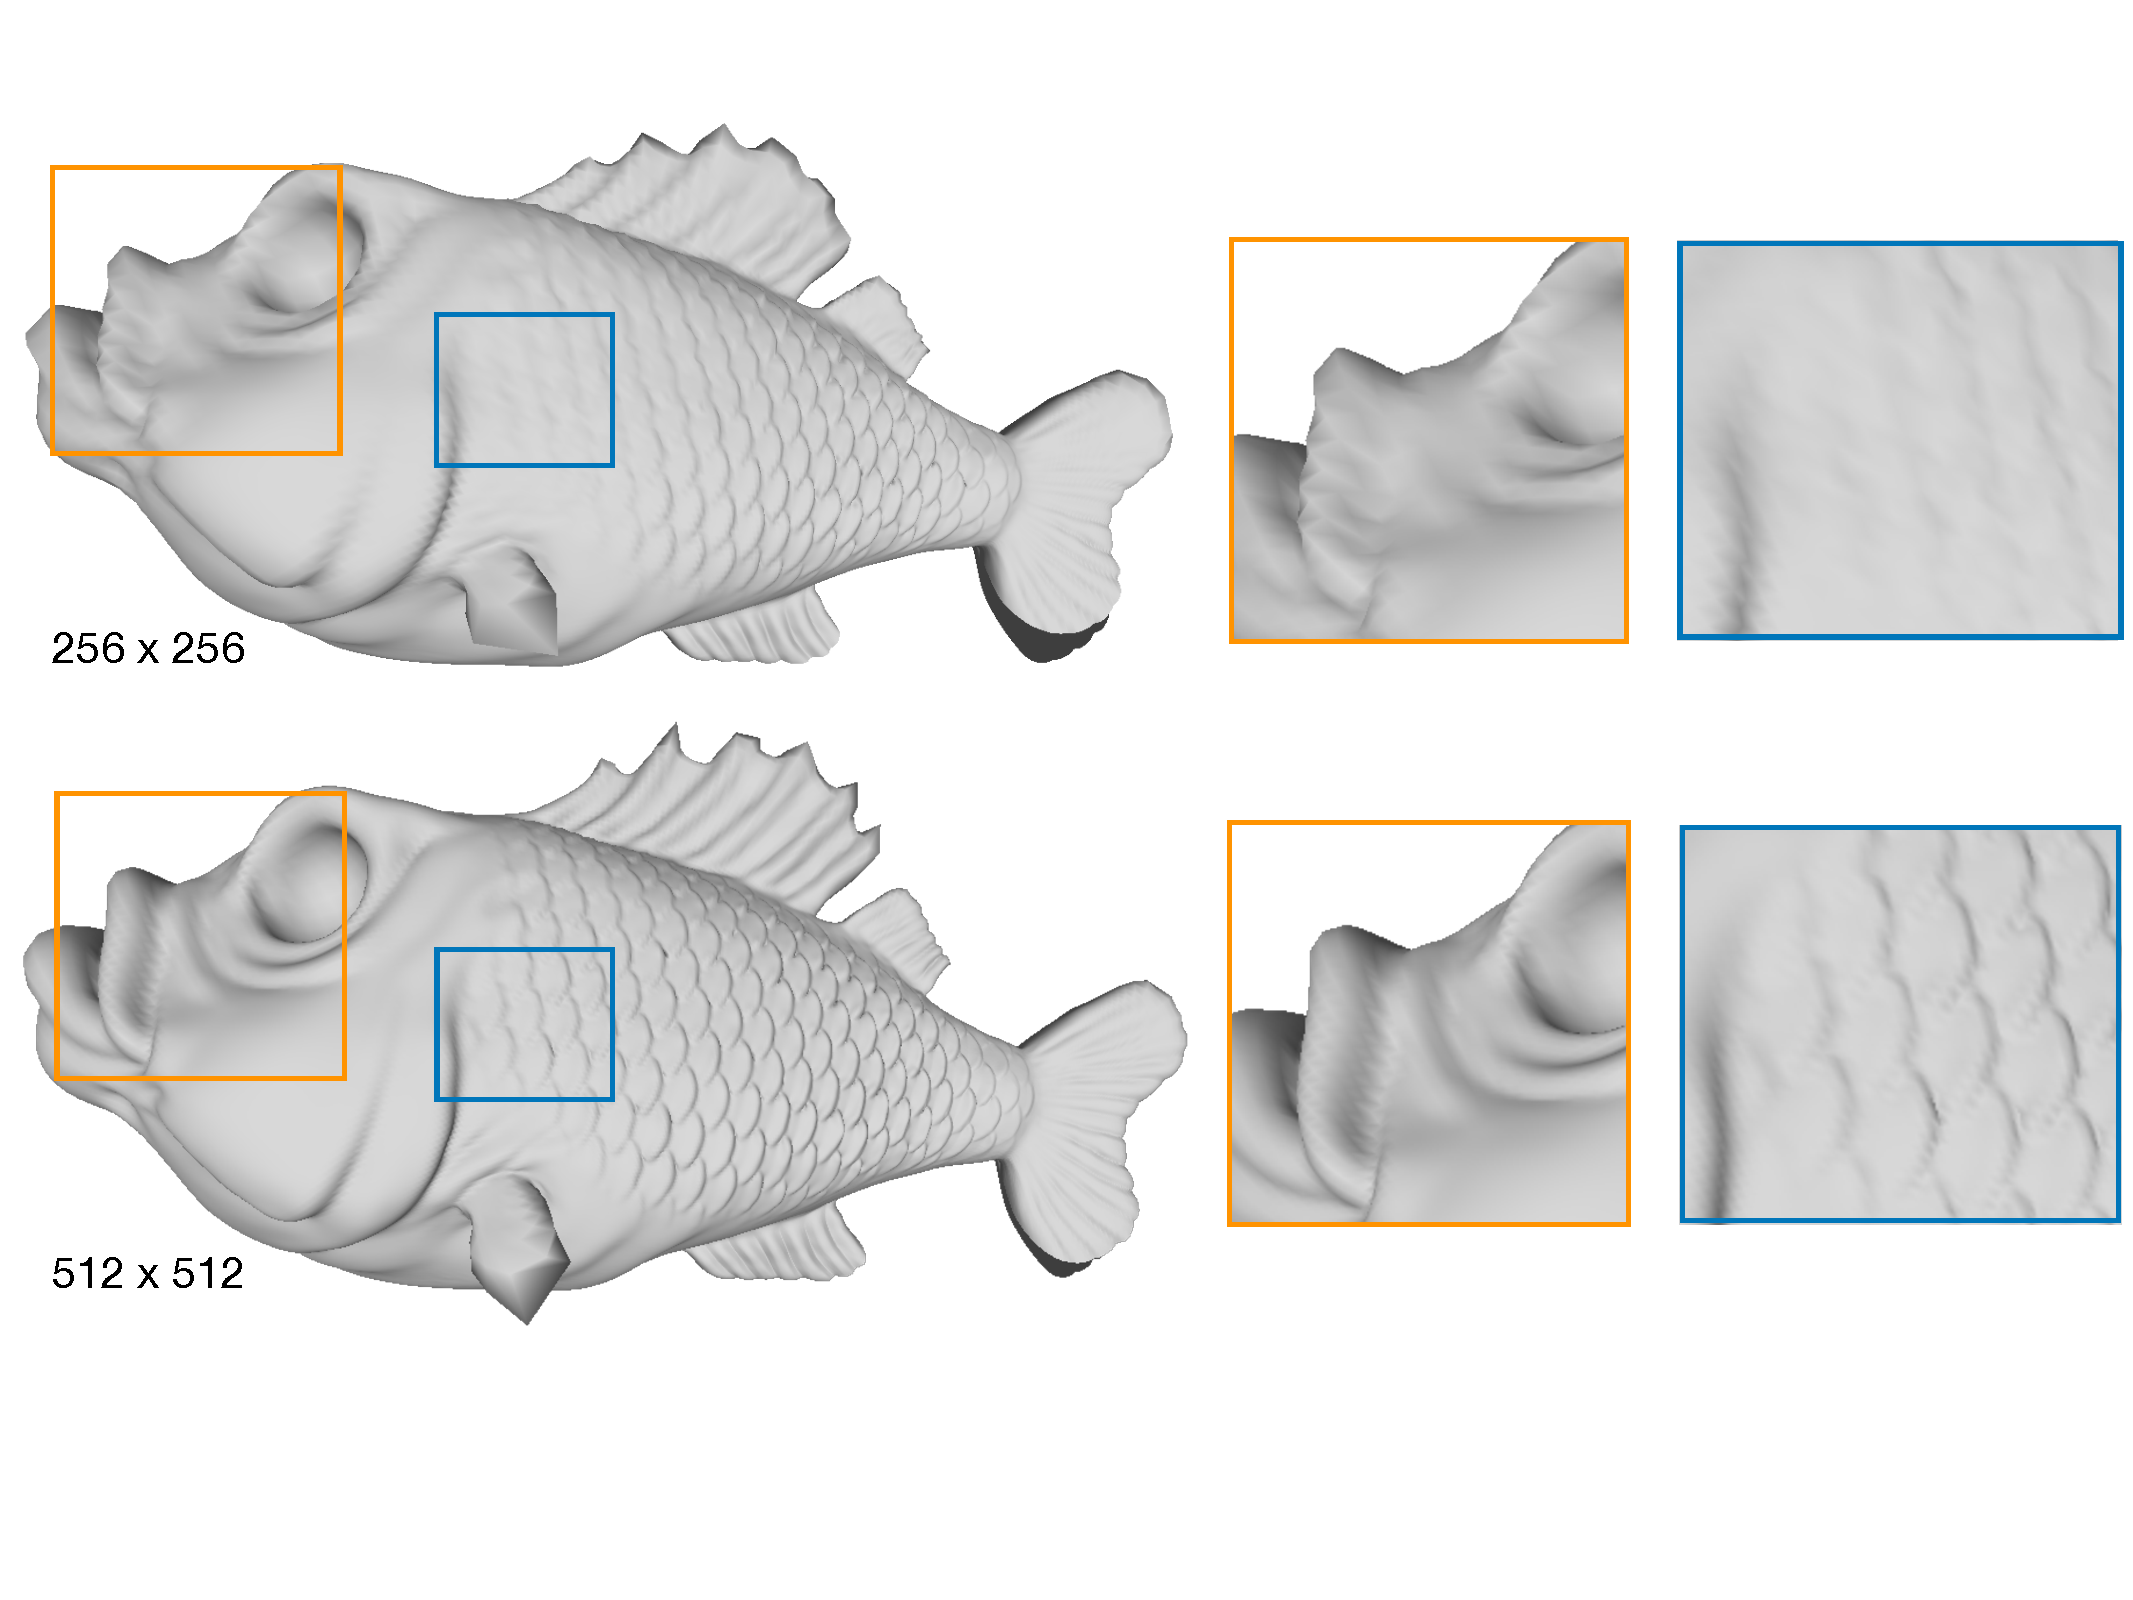
\includegraphics[width=0.5\textwidth]{Figures/fish}
     \caption{Fish reconstructions after uniform-resampling of Harmonic Map}
     \label{Fig: Fish Reconstruction}
\end{figure}
%------------------
% FIGURE (Varying Lighting)
\begin{figure}[H]
  \centering
    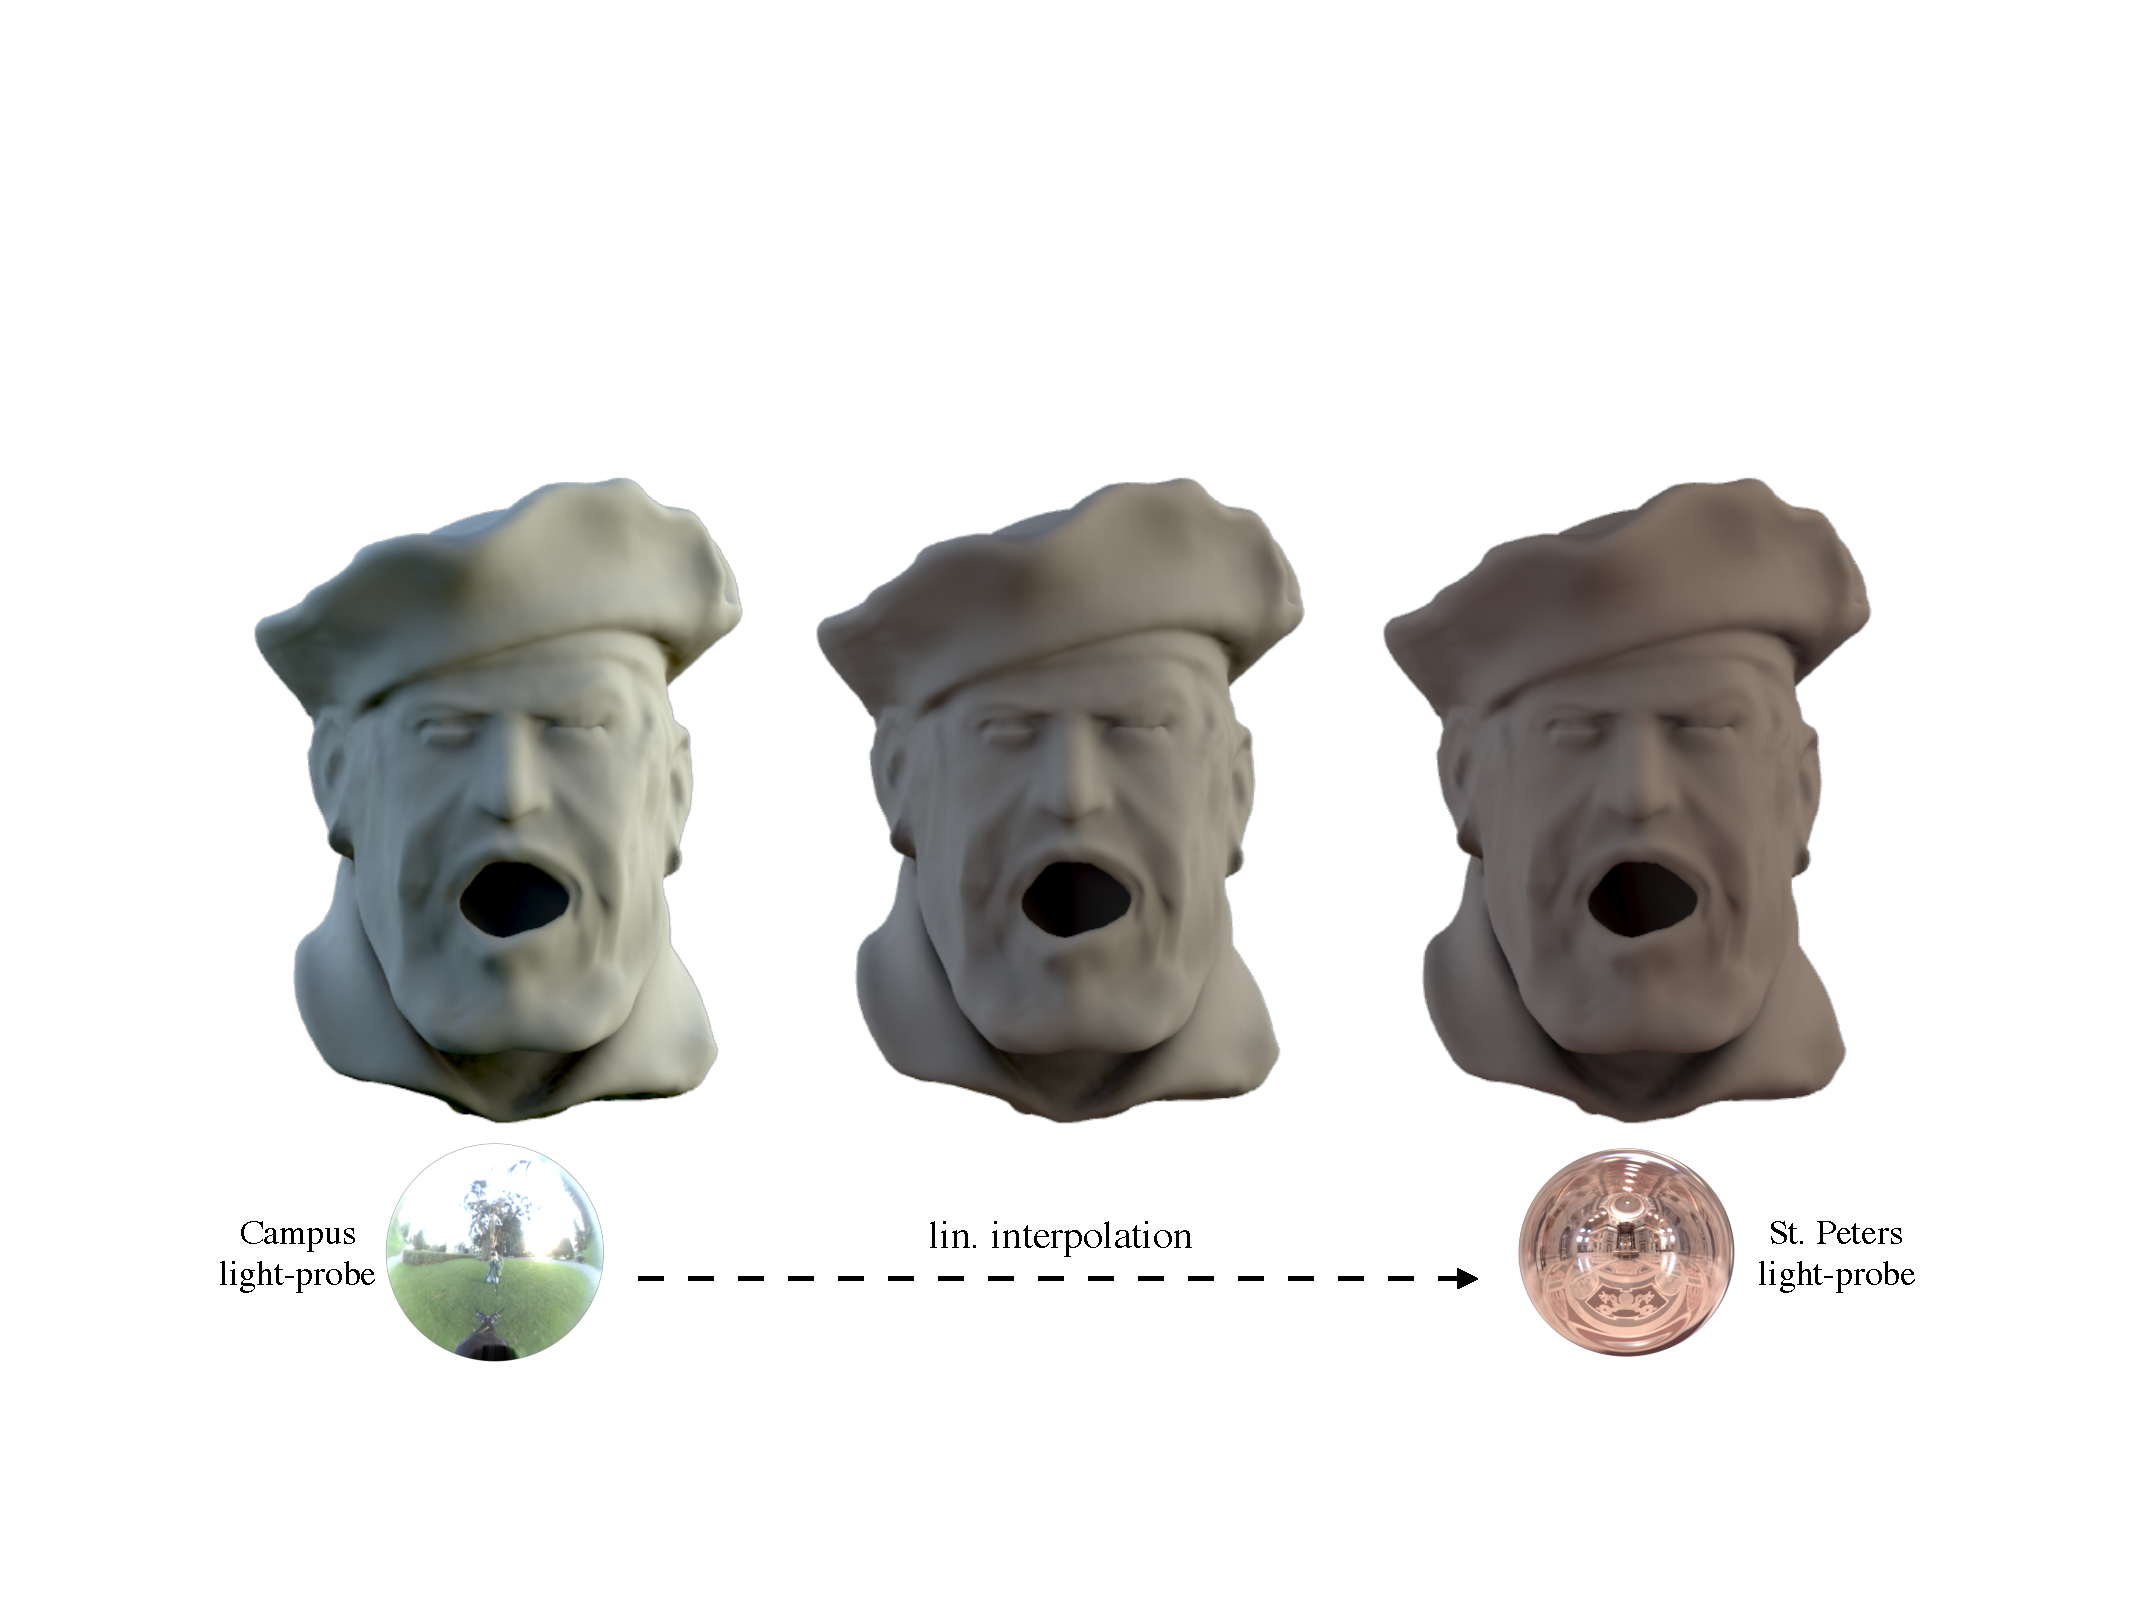
\includegraphics[width=0.4\textwidth]{Figures/varying_lighting}
     \caption{Method is independent of lighting condition}
     \label{Fig: Varying lighting}
\end{figure}
%------------------
%%%%%%%%%%%%%%%%%%%%%%%%%%%%%
% MEMORY and QUALITY
%%%%%%%%%%%%%%%%%%%%%%%%%%%%%
\subsection*{Memory Savings}
For each of the test objects, our training sets comprises 450 distinct object deformations. \\
Now, for demonstration purposes, lets assume the shapes of this training set are precisely the target shapes which appearances are requested to be computed for a given application.
\\
Within that training set, our CNN model is able to achieve accuracies up to 98\% (table \ref{Table: NN_Accuracy}) and its rendered appearances become visually indistinguishable from the ground truth (Figure (\ref{Fig: DPRT_Quality}) ). 
This means, that our trained network is able to faithfully generate self-shadowing effects of 450 distinct shapes \textbf{at the very least}, only requiring the storage of the network parameters.
\\ 
On the contrary classic PRT would imply storing the transfer coefficients of each vertex for every single shape of the training set.
\\ 
For our particular network of approx. $11,8$ million parameters,  the example objects with $256 \times 256$ and $512 \times 512$ number of vertices, and  a choice of 16 transfer coefficients per vertex, this implies a compression ratio of: 
\begin{align*}
r = \frac{\text{\# PRT-params}}{\text{\# CNN-params}}  = 
\begin{cases}
\textbf{40,022} , & \mbox{for } 256^2 \mbox{ \#vertices} \\
\textbf{160,088} & \mbox{for } 512^2 \mbox{ \#vertices}
\end{cases}
\end{align*}
This number grows linearly with increasing number of coefficients, number of deformations or number vertices. 
%%%%% TABLE %%%%%%%%%%%
\begin{table}[H]
\begin{tabular}{|l|l|l|l|l|}
\hline
\textbf{}            & \textbf{Accuracy} & \textbf{Loss} & \multicolumn{2}{l|}{\textbf{Val-Loss}} \\ \hline
\textbf{Pirate Head} & 0.9817            & 0.000397            & \multicolumn{2}{l|}{0.000399}                 \\ \hline
\textbf{Fish}        & 0.9729            & 0.002104            & \multicolumn{2}{l|}{0.002200}                 \\ \hline
\textbf{Cloth}       & 0.9818            & 0.000786            & \multicolumn{2}{l|}{0.000907}                 \\ \hline
\end{tabular}
\caption{Network Accuracy}
\label{Table: NN_Accuracy}
\end{table}
%%%%%%%%%%%%%%%%%%%
The numbers shown above express the compression ratio taking into account solely the training set. On top of that, our network shows good generalisation properties, also enabling accurate and qualitatively precise appearance predictions of deformations outside the training set. Thus, by taking this into account the compression ratio grows to immeasurable values. 
\\
Thus, we show that DeepPRT, as it is, is capable of drastically diminishing the storage consumption of PRT algorithms for deforming objects. 
\\
As mentioned above, commonly deep convolutional networks itself can be highly optimised, hence making DeepPRT even much more efficient, energy, speed and memory wise \cite{Survey_NN_Compression}. 
%%%%%%%%%%%%%%%%%%%%%%%%%%%%%
% Comparisson 
%%%%%%%%%%%%%%%%%%%%%%%%%%%%%
\subsection*{Generality of DeepPRT and Comparison}
\subsubsection*{Generalisation Capability:}
We validate the generalisation capabilities of our model by standard machine learning procedures. We base our parameter tuning on minimising the validation loss and later analyse prediction quality using a test set.\\ 
The results show small errors and are in most cases visually indistinguishable or close to the ground truth (Figure [??]). 
\begin{figure}[H]
  \centering
    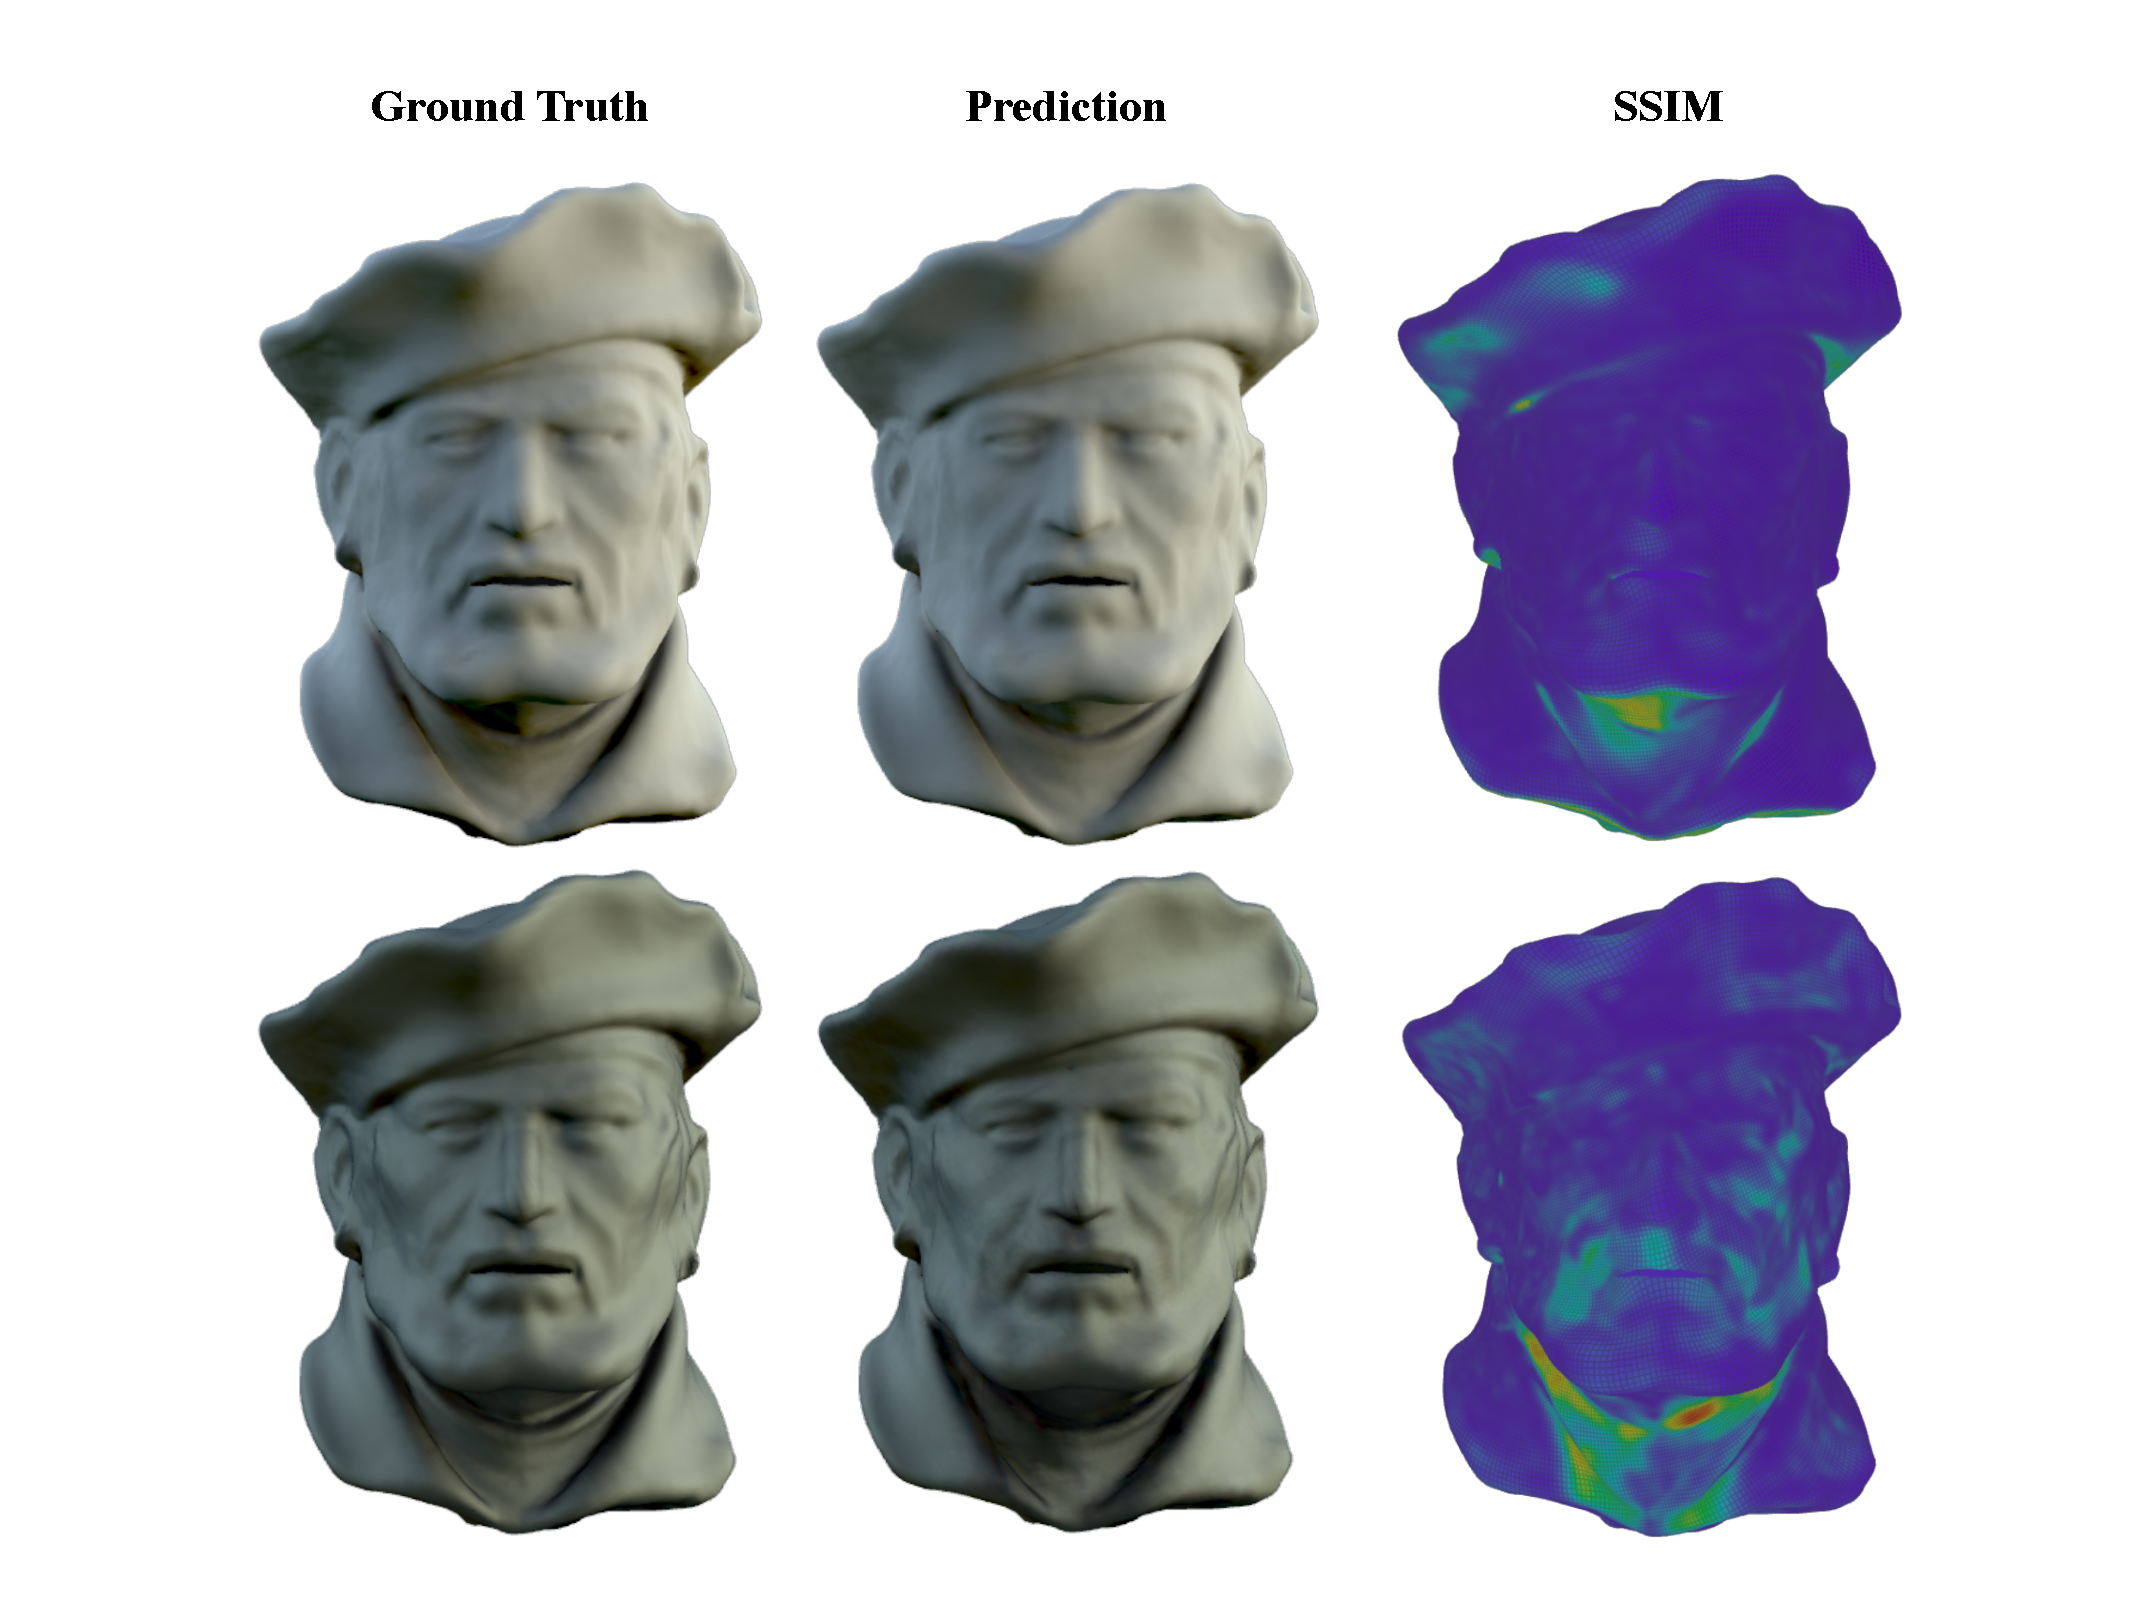
\includegraphics[width=0.35\textwidth]{Figures/glossy_pirate.pdf}
     \caption{Example: glossy pirate}
     \label{Fig: glossy_pirate}
\end{figure}
\subsubsection*{\textbf{Comparison with MoMoPRT}~:}
Furthermore, we compare our method with \cite{MoMoPRT} (MoMoPRT) and show that DeepPRT it is more accurate and can handle more general deformations. \\
The authors of \cite{MoMoPRT} proposed a linear model $f_{lin}$ to predict transfer coefficients within a "linear shape space", namely the space spanned by a Morphable Model.\\
This approach is clearly limited to shape deformations that are contained within the space described by the linear-shape-model $S_{lin}$ of choice. Moreover, although a linear model may be enough to approximate self-shadowing effects of shapes that are close to the mean shape of the training-data-distribution, the model lacks complexity to accurately approximate data samples that exist farther away from the mean shape (underfitting).  
\\
On the other hand, our more complex non-linear CNN model ($f_{CNN}$) is able to capture the relationships between the dataset's features (shape) and the target variable (transfer coefficients), enabling accurate approximations for a much larger deformation domain.\\
\\
For demonstration purposes, we generate a new training set consisting of, randomly sampled, linear combinations between visually more dissimilar basis shapes\footnote{More distinguishable between each other, than between each face expressions used in \cite{MoMo}.}: 1) the \textit{Pirate Head } on one side, and 2)  a simple \textit{Plane} on the other. We train both models, $f_{CNN}$ and $f_{lin}$, and compute their predictions for a series of test-shapes that are evenly distributed over the linear shape space. Figure (\ref{Fig:DPRT vs MoMoPRT A}) shows that the prediction accuracy of our $f_{CNN}$ model is higher and remains almost constant over the entire domain; on the contrary, the prediction accuracy of the linear model $f_{lin}$ drops significantly moving away from the mean shape (the \textit{Pirate/Plane} hybrid), as expected. 
\begin{figure}[h]
  \centering
    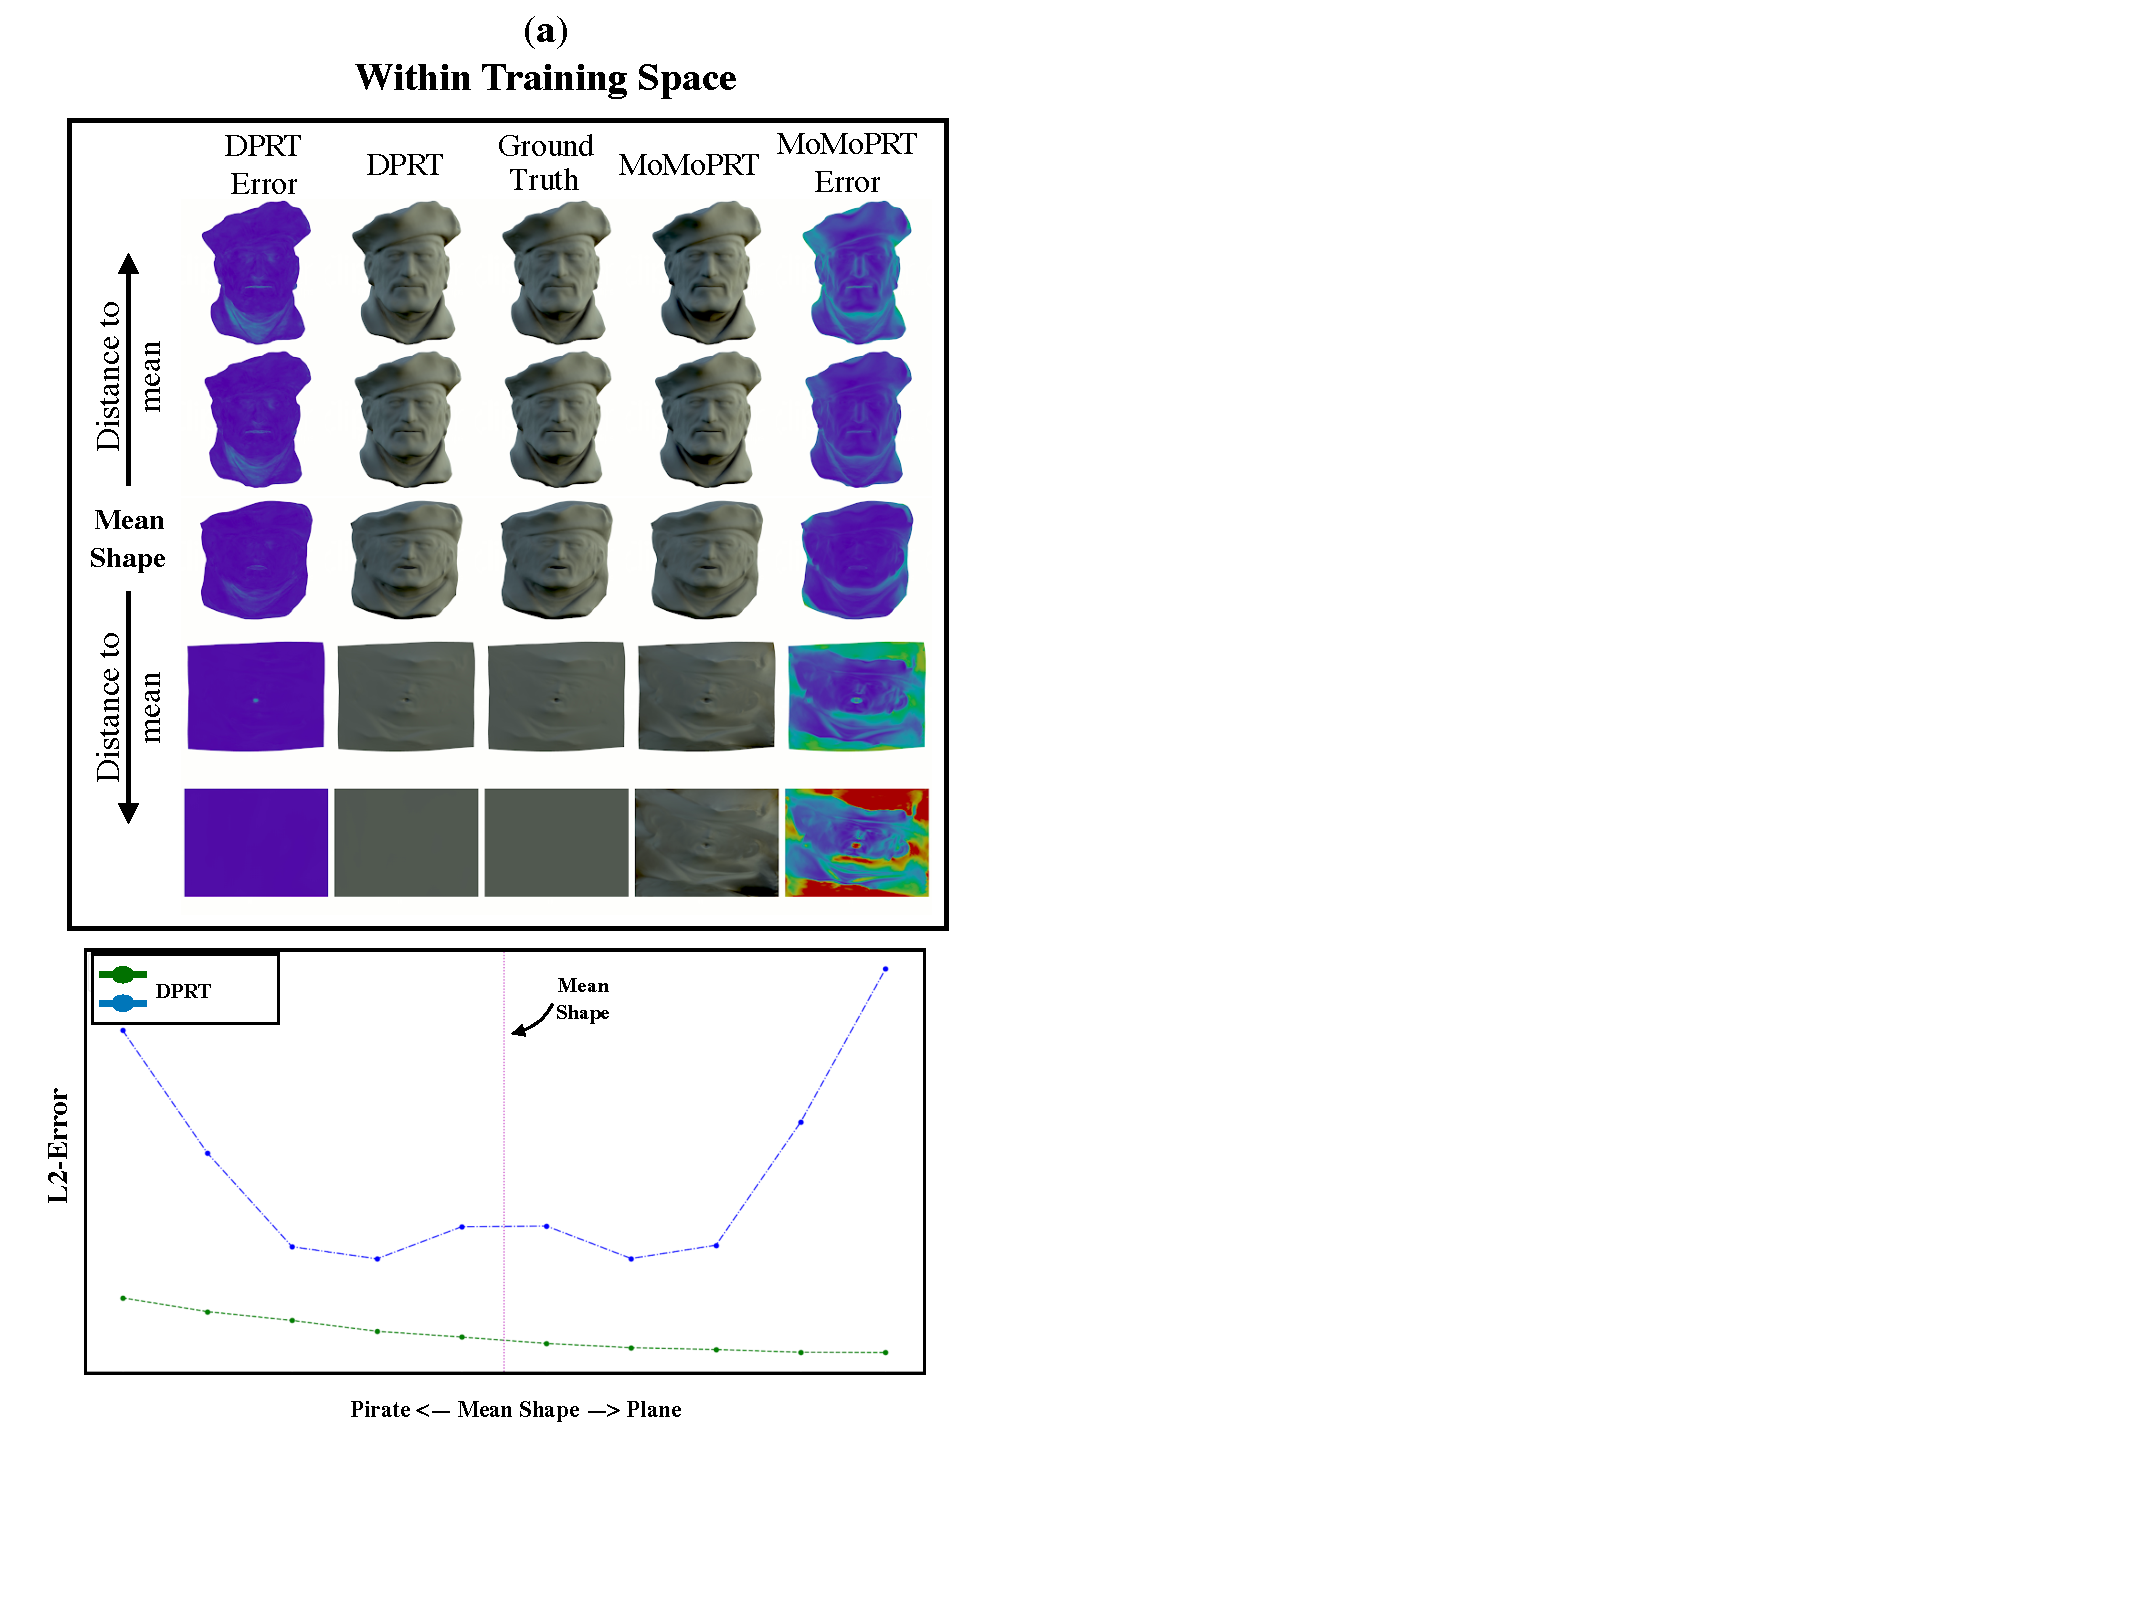
\includegraphics[width=0.4\textwidth]{Figures/DPRT_vs_MoMoPRT_a.pdf}
     \caption{Example: DPRT vs MoMoPRT}
     \label{Fig:DPRT vs MoMoPRT A}
\end{figure}
Last but not least, we demonstrate that our model approximates data that is contained in a much larger domain than the one spanned by a linear-shape-model $S_{lin}$. The models, $f_{CNN}$ and $f_{lin}$, are fed with a series of sample shapes, starting from the mean shape and increasingly deforming towards a \textit{Pirate} face expression that was excluded from the training set. \\
As can be seen in Figure (\ref{Fig:DPRT vs MoMoPRT B}), the linear model is not able to predict shapes away from its shape-space $S_{lin}$, while our method, again shows a close to constant prediction accuracy.
\begin{figure}[h]
  \centering
    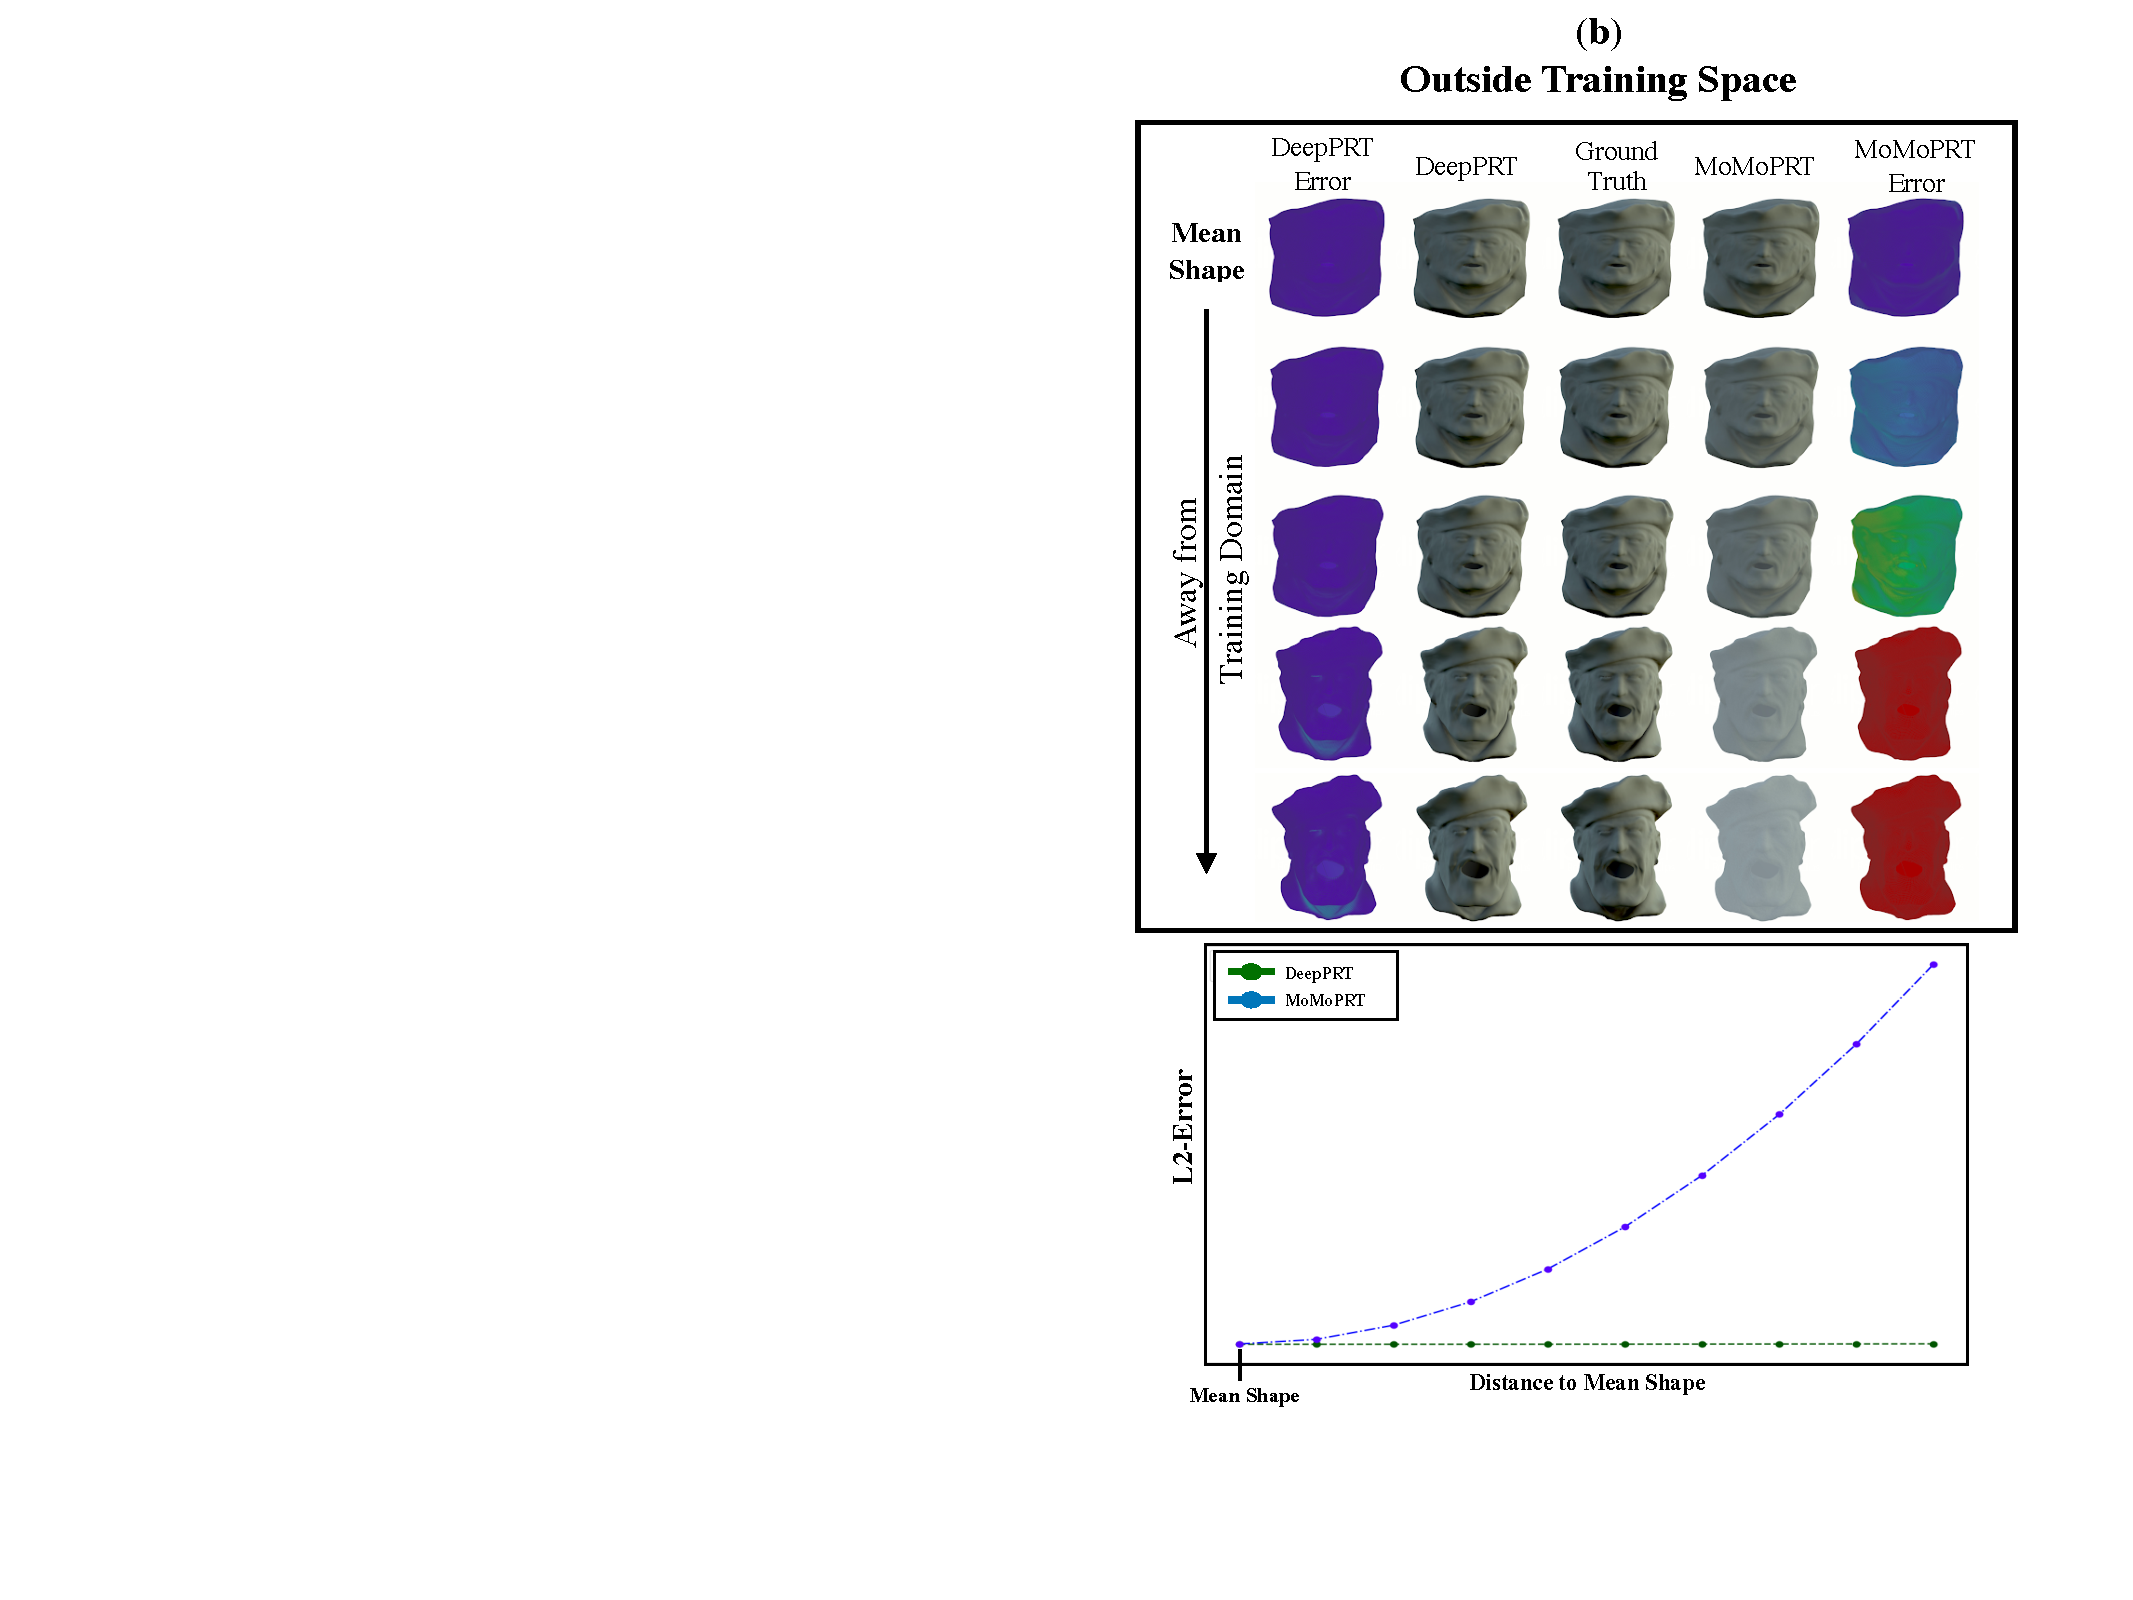
\includegraphics[width=0.4\textwidth]{Figures/DPRT_vs_MoMoPRT_b.pdf}
     \caption{Example: DPRT vs MoMoPRT}
     \label{Fig:DPRT vs MoMoPRT B}
\end{figure}

